\documentclass[12pt,oneside,english]{article}

\usepackage[T1]{fontenc}
\usepackage[latin1]{inputenc}
\usepackage{geometry}
\geometry{verbose,letterpaper,tmargin=1in,bmargin=1in,lmargin=1in,rmargin=1in}
\usepackage{textcomp}
\usepackage{babel}
\setcounter{secnumdepth}{0}
\usepackage{graphicx}
\usepackage{float}
\floatstyle{boxed}
\restylefloat{figure}
\usepackage{longtable}
\usepackage{url}

\newcommand{\BibTeX}{{\sc Bib}\TeX}


\begin{document}
\sffamily

        \title{in-situ impedance and morphology of self-assembling gold nanoislands}

	\author{John Donovan, Dr. Chuhee Kwon\\
	University of California, Long Beach, CA\\
	{\small donovan.csulb@gmail.com ckwon@csulb.edu}}
	
        \date{\today}

	\maketitle


        \section{Introduction}

	\begin{figure}
	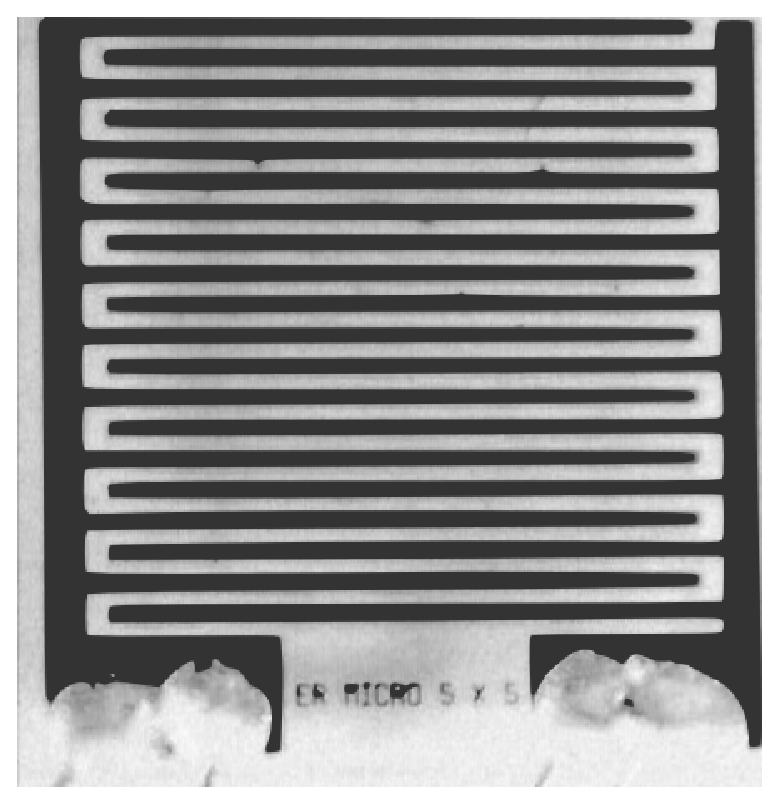
\includegraphics[scale=0.4]{images/IDE.eps} \label{f:IDE}
	\caption{The self-assembling gold monolayers are deposited on a gold inter-digitized electrode (IDE).}
	\end{figure}
	
	\subsection{background}
	Gold nanoislands  are formed by annealing a substrate -- on which gold has been uniformly deposited -- to produce islands within a predictable range of size and shape.
	

	\subsection{purpose}
	This research attempts to create reproducible samples of gold nano-islands and study their morphology.
	Prior research suggests that the physical properties of gold nano-islands are sensitive to the method of depositing the gold, the number of layers, and variations in annealing temperature \cite{shon07}.  
	Gold nano-island formation through polymer-assisted self-assembly is also sensitive to the initial size of the colloidal gold used to form the self-assembling layers \\cite(reference), to the temperature profile during annealing, and to the length of time (in days) between creation and annealing (\cite{joshi}).
	This research quantifies the repeatiblity of gold nano-islands produced using the label-free(*) self-assembly method.

	\subsection{method}
	Samples are produced using polymer-assisted self-assembling monolayers.

	\section{Procedure}

	\subsection{The Chemistry of Self-Assembling Films}
	
	\emph{COMMENT: This section is based on discussion with YS Shon, and attribution should be made for these ideas.}
	
	Gold self-assembling films were produced from two sizes of gold particle.  
	The larger particles were Au$_{314}$, the smaller were Au$_{25}$.  
	These particles are coated in different organic ligands, which aid their solubility in ethanol (in the case of Au$_{314}$) and water (in the case of Au$_{25}$).    
	The ligands are terminated with a carboxy group (COOH) in ethanol and aqueous solutions; in the aqueous Au$_{25}$ solution, ligands may also be terminated with a positively charged carboxy group (COO-). 
	
	After the first gold layer is deposited the sample is dipped in an aqueous solution of Poly(allylamine hydrochloride) (PAH).  
	The PAH bonds to the ligands and allows the next layer to assemble.  	
	The aqueous PAH molecules are terminated with amine groups (NH$_2$) and with positively charged amine groups (NH$_3^+$).  
	The relative occurrence of the NH$_3^+$ groups determine the pH of the solution.
	
	In the aqueous Au$_{25}$ solution, the PAH NH$_3^+$ group favorably bonds to the ligand COOH and COO- groups.
	The density of the single self-assembled gold layer therefore depends (non-linearly) on the pH of the PAH solution, with lower pH (higher ratio of NH$_3^+$ groups) resulting in higher packing density.
	The effect of pH on Au$_{25}$ layer density may be studied in this or another paper.
	
	In the ethanol Au$_{314}$ solution, there is an absence of ligand COO- groups.
	A more neutral pH of the PAH solution allows more bonds between NH$_2$ and COOH groups.
	
	\subsubsection{A model of gold density in Au$_{314}$ and Au$_{25}$ films}
	The difference in gold density between self-assembling Au$_{314}$ and Au$_{25}$ films can be visually observed.
	In previous unpublished study, an gold film formed from 8-layers of self-assembled Au$_{25}$ was equivalent in color to a Au$_{314}$ film of approximately 2-4 layers.
	The relationship between color and gold film thickness is a well-documented one, for films deposited by evaporation.
	If instead the color of a nano-island film is observed, the color may be misleading, as nano-island phonons depend not just on thickness, but also size and shape of the islands.  
	The size and shape of nano-islands depends on factors that include the initial size of the colloidal gold.
	
	To reach a first-order approximation of the relative gold density of Au$_{314}$ and Au$_{25}$ films, some assumptions must be made.
	First, the average length of the ligands are assumed to be fixed (we neglect that these ligands can easily stretch or shrink).
	Also, the effect of the pH in the PAH solution on packing density should be considered a second-order effect until demonstrated otherwise.	
	
	[image in which the gold particles are modeled as packed spheres]	
	
	The approximate ligand length is 2${\mu}m$ for Au$_{314}$ and approximately 1${\mu}m$ for Au$_{25}$.
	The approximate size of the colloidal gold particles are 2.5${\mu}m$ for Au$_{314}$ and 1${\mu}m$ for Au$_{25}$.
	Making the assumption that these particles can be modeled as spheres of radius 3${\mu}m$ for Au$_{314}$ and 1.5${\mu}m$ for Au$_{25}$ leads to a relative density of 4 nanoparticles of Au$_{25}$ per nanoparticle of Au$_{314}$, which yields an approximate density of 100/314.
	
	At the first order, three times more layers of Au$_{25}$ should therefore be deposited to yield an equivalent gold mass to the Au$_{314}$ film.
	
	In real application, thermolysis of much more than 8 layers of a film will result in defects of significant density to affect the production of our nanoislands of interest.
	It is therefore better to use larger Au$_{314}$ particles instead of many layers of Au$_{25}$.

	\subsection{Size and Shape Distributions and Phonon Absorption Features}
	The uniformity of the size and shape is expected to correlate with the width of the absorption feature of the resulting sample.
	A wider distribution of sizes and shapes is expected to produce a broader absorption peak, while a narrower distribution of nanoisland sizes about the average size is expected to produce a sharper absorption feature.
	This relationship is predicted analytically because identical islands should absorb identically (neglecting second-order effects), producing a maximized peak.  
	Differences among the islands will create phonons that are offset by some amount from the peak wavelength, resulting in a lower and broader peak.
	


	\subsection{Measurement of Complex Impedance}
	DC resistance measurements of the electrode show only its insulating properties, as the glass substrate is a poor conductor and the IDE is a weak capacitor, so AC resistance is measured.
	AC resistance is also shown to follow the temperature-dependent electron mobility.
	
	\begin{equation}
		R = R_0 cdot \exp{\epsilon\over{k cdot T}}
		\label{eq:emobility}
	\end{equation}
	
	Sample resistance (a parallel AC resistance) is typically high for the sample under test, this resistance changes when the sample is heated and the polymers are burned off.  

	The resistance $R_p$ of a high-resistance sample can be measured from the complex impedance $(Z,\theta)$ by Equation ~\ref{eq:R_p}.  Use of the parallel resistance $R_p$ is justified at high sample resistance because the series resistance $R_s$ of the test leads and contacts are orders of magnitude smaller.
	
	\begin{equation}
		R_p = {{Z} \over {cos({\theta})}}
		\label{eq:R_p}
	\end{equation}
	
	Typical values for complex impedance measured by the auto-balancing bridge method via an Agilent 82XX LCR meter are as follows.
	
	\begin{equation}
		\left( Z,\theta,\nu,T \right) = \left( 15 M\Omega, -89.9^\circ, 1kHz, 22^{\circ}C \right)
	\end{equation}
	\begin{equation}
		\left( Z, \theta, \nu, T \right) = \left( 800 k\Omega, -88^\circ, 45kHz, 22^{\circ}C \right)
	\end{equation}
	
	This result shows that the $R_p$ ``resistance'' component (which is $Z$ divided by $cos(-89^\circ)$) is immeasurably high at low frequencies and low temperature.  It is only at higher temperatures that $R_p$ drops to the measurable range, and this occurs at about $250^{\circ}C$ when the impedance phase angle $\theta$ drops from $-89.9^\circ$ towards $0.1^\circ$.
	
	During the burn-off of the polymers, the parallel resistance may drop to under 100 ohms, which requires a four-point measurement to compensate for the series resistance test lead impedance.
	A four-point measurement is necessary because the test leads have been reported (AD5933) to have up to kilo-ohm impedance when measuring low sample resistance.


\clearpage
\bibliography{thesis_draft}
\bibliographystyle{plain}


\end{document}
%% The following is some template materials -- equations and figures.
\documentclass[aps,prl,twocolumn,oneside,showkeys,floatfix]{revtex4-1}
\newcommand{\BibTeX}{{\sc Bib}\TeX}
\usepackage{graphicx}
\usepackage{listings}

\newbox\bwk\edef\tempd#1pt{#1\string p\string t}\tempd\def\nbextr#1pt{#1}
\def\npts#1{\expandafter\nbextr\the#1\space}
\def\ttwplink#1#2{\special{ps:1 0 0 setrgbcolor}#2\special{ps:0 0 0 setrgbcolor}\setbox\bwk=\hbox{#2}\special{ps:( linkto #1)\space\npts{\wd\bwk} \npts{\dp\bwk} -\npts{\ht\bwk} true\space Cpos}}
        \begin{equation}
        \nu_{\mathtt{Larmor}} = {{\Delta E} \over{ 2 \pi \hbar}} = {{2 B \cdot \mu_{\mathtt{proton}}} \over{2 \pi \hbar}}
        \end{equation}

        \author{John \surname{Donovan}}
        \affiliation{CSULB}
        \begin{abstract}
                \begin{description}
                        \item[Background] This part would describe the
                        context needed to understand what the paper
                        is about.
                        \item[Purpose] This part would state the purpose
                        of the present paper.
                        \item[Method] This part describe the methods
                        used in the paper.
                        \item[Results] This part would summarize the
                        results.
                        \item[Conclusions] This part would state the
                        conclusions of the paper.
                \end{description}
        \end{abstract}
        \keywords{nano,nano-islands,thin films}
        \maketitle
        Written in \LaTeX\ with TexMaker.


\begin{figure}
\includegraphics[scale=0.5]{BField_Set1.eps} \label{BSet1}
\caption{The magnetic field (in MHz resonance frequency) measured.  Set 1 did not include many measurements of the most uniform part of the field.}
\end{figure}

\clearpage
\begin{widetext}
\section{Appendix}
\subsection{Spin Echo Peak-Finder Algorithm in Matlab}
\lstset{language=Matlab, basicstyle=\footnotesize, numbers=left, captionpos=t, breaklines=true, caption=find\_spin\_echo() locates the pulse maxima in a spin-echo pulse train, label=T2 Pulse Train, frame=shadowbox}
\lstset{basicstyle=\small\ttfamily, basewidth=0.51em}
\lstinputlisting{../find_pulse_train.m}
\end{widetext}


